\section{Problem Formulations and NP-Completeness Proofs}
\label{sec:problem-analysis}

In this section we define three PMU placement problems: \maxinc (Section \ref{subsec:maxinc}), \xval (Section \ref{subsec:xval}), and \xvalpart (Section \ref{subsec:xvalpart}). 
For each problem, we first define the optimization version of the problem and then its corresponding decision problem.  Finally, we prove that each decision problem is NP-Complete.
Note that in all three placement problems we are only concerned with computing the voltage phasors of each bus. Using the values of the voltage phasors, 
Ohm's Law can be easily applied to compute the current phasors of each transmission line.

\subsection{Proof Strategy}
\label{subsec:proofstrat}
In the coming sections we use slight variations of the approach presented by Brueni and Heath in \cite{Brueni05} to prove the NP-completeness of the problems we consider. 
We found their scheme to be extensible for proving many properties of PMU placements. For purposes of clarity, we begin by explaining this approach in general terms,
and then consider the approach in detail for each problem.

Our NP-Completeness proofs all reduce from planar 3-SAT (\sats). A \sat formula, $\phi$, is a boolean formula in conjunctive normal form (CNF) such that each clause contains at most $3$ literals and 
the undirected graph $G(\phi)$ is planar \cite{Lich82}. %\cite{Garey79}. 
$G(\phi)=(V(\phi),E(\phi))$ is a bipartite graph constructed from a 3-SAT formula $\phi$ with variables $\{v_1,v_2, \dots , v_r\}$ and the set of clauses $\{c_1,c_2, \dots , c_s \}$ as follows: 
$V(\phi) = \{v_i$ $\vert$ $1 \leq i \leq r \} \cup \{c_j$ $\vert$ $1 \leq j \leq s \}$ and $E(\phi) = \{ (v_i,c_j)$ $\vert$ $v_i \in c_j$ or $\overline{v_i} \in c_j\}$.
For example, \sat formula
\begin{eqnarray}
	 \varphi &=& (\overline{v_1} \vee v_2 \vee v_3) \wedge (\overline{v_1} \vee \overline{v_4} \vee v_5) \wedge (\overline{v_2} \vee \overline{v_3} \vee \overline{v_5}) \nonumber\\ 
	 & & \wedge (v_3 \vee \overline{v_4}) \wedge  (\overline{v_3} \vee v_4 \vee \overline{v_5}) 
\label{eqn:varphi}
\end{eqnarray}
has graph $G(\varphi)= (V(\varphi),E(\varphi))$ shown in Figure \ref{fig:gvarphi}.  Note that $\varphi$ is a specific \sat formula used for this example and is thus
different from the generic \sat formula, $\phi$, used in our reductions.

Following the approach in \cite{Brueni05}, for \sat formula, $\phi$, we replace each variable node and each clause node in $G(\phi)$ with a specially constructed set of nodes, 
termed a {\em gadget}. Specifically, each variable gadget has a subgraph of nodes that represent a ``True" assignment to that variable, and a subgraph of nodes that represent a ``False" assignment to the variable.
All variable gadgets have the same structure, and all clause gadgets have the same structure (that is different from the variable gadget structure).
We then prove that a PMU placement for this graph results in a fully (maximally) 
observed graph if and only if that PMU placement can be interpreted as assigning unambiguous truth values to each variable, in a manner which satisfies the formula $\phi$.
For convenience, when we refer to reference \cite{Brueni05}, we are alluding to Theorem 9 in \cite{Brueni05}.

%the problem exactly. NP-Complete problems are the hardest problem in completixty class $\mathcal{P}$.  Showing a problem is NP-Complete is a two step procedure: (1) show that a solution
%to the problem can be verified in polynomial time and (2) all known NP-Complete problems are at least as hard as $L$.  Step (2) is done through a reduction: .

\begin{figure}[t]
\centering
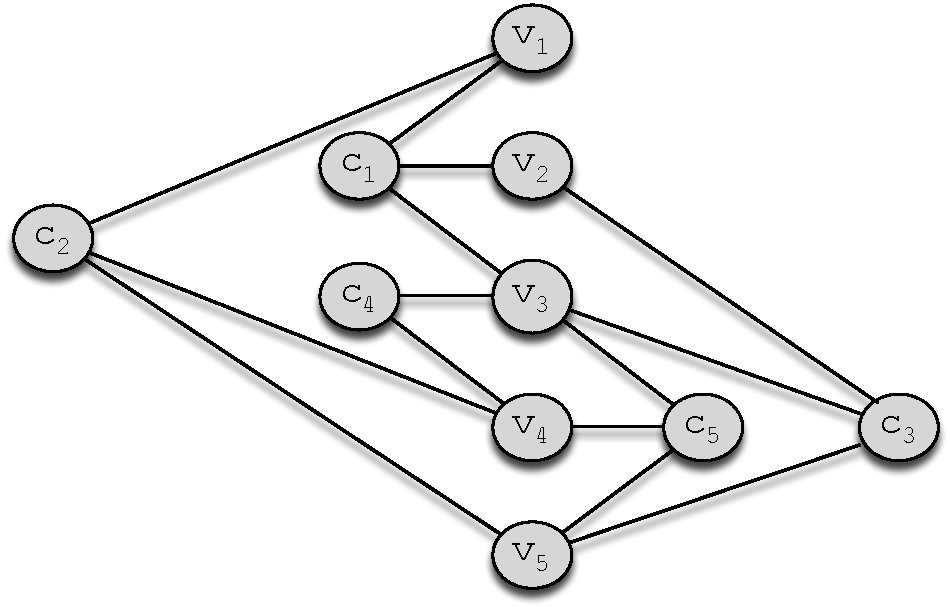
\includegraphics[scale=0.55]{figs/gvarphi.pdf}
\caption{$G(\varphi)=(V(\varphi),E(\varphi))$ formed from $\varphi$ in Equation (\ref{eqn:varphi}) }
\label{fig:gvarphi}
\end{figure}


\subsection{\maxinc Problem Statement}
\label{subsec:maxinc}

%Here we define both an optimization and decision version of the \maxinc problem. 
\maxinc is a variation of the PMUP problem described by Brueni and Heath \cite{Brueni05} and the PDS problem defined by Haynes et al. \cite{Haynes02}: rather
than consider the minimum number of PMUs required for full system observability, \maxinc finds the maximum number of nodes that can be observed using a fixed number of PMUs.

%Before formally stating the \maxinc problem, we present some notation.
%Let $k^*$ be the minimum number of PMUs needed for $\Phi^R = V$. Let $\Phi^R_G$ and $\Phi^R_{G'}$ be the observed nodes for graph $G$ and $G'$, respectively. Finally, $m$ is a
%constant corresponding to a graph $G=(V,E)$ such that $m < |V|$. 

\maxinc Optimization Problem: 
\begin{itemize}
	%\textsc{Input}: Graph $G=(V,E)$, $k$ PMUs such that $1 \leq k < k^*$.
	\item \underline{Input}: Graph $G=(V,E)$, $k$ PMUs such that $1 \leq k < k^*$.

	\item \underline{Output}: A placement of $k$ PMUs, $\Phi$, such that $|\Phi^R_G|$ is maximum.
	%\textsc{Output}: A placement of $k$ PMUs, $\Phi$, such that $|\Phi^R|$ is maximal.
\end{itemize}

\maxinc Decision Problem: 
\begin{itemize}
	\item \underline{Instance}: Graph $G=(V,E)$, $k$ PMUs such that $1 \leq k < k^*$.

	\item \underline{Question}: For a given $m< |V|$, is there a $\Phi_G$ such that $|\Phi_G| \leq k$ and $m \leq |\Phi^R_G| < |V|$?
	%\item \underline{Question}: Is there a $\Phi \subseteq V$ such that $|\Phi| \leq k$ and $m \leq |\Phi^R| < |V|$?
\end{itemize}



Before proving that \maxinc is NP-Complete, we provide some background on NP-Completeness. NP-Complete problems are the hardest problems in complexity class $\mathcal{NP}$. 
%Additionally, for an NP-Complete problem, $\Pi$, there is no known polymonial time algorithm to solve $\Pi$ exactly in all instanstces. 
Proving a decision problem, $\Pi$, is NP-Complete is a three step procedure. First, we need to show $\Pi$ is in $\mathcal{NP}$. Second, we select a known NP-Complete problem $\Pi'$
and construct a polynomial-time transformation, $f$, that maps any instance of $\Pi'$ to an instance of $\Pi$. 
Finally, we need to prove that $f$ is a transformation: $f$ maps any ``yes'' instance of $\Pi'$ to a ''yes'' instance of $\Pi$ and any ''no'' instance of $\Pi'$ to a ``no'' instance 
of $\Pi$ \cite{Garey79}. %vice versa. 

% Our NP-Completeness proof for \maxinc reduces from \sats. A \sat formula, $\phi$, is a boolean formula in conjunctive normal form such that each clause contains at most $3$ literals and 
% the undirected graph $G(\phi)$ is planar \cite{Lich82}. %\cite{Garey79}. 
% $G(\phi)=(V(\phi),E(\phi))$ is a bipartite graph constructed from a 3-SAT formula $\phi$ with variables $\{v_1,v_2, \dots , v_r\}$ and the set of clauses $\{c_1,c_2, \dots , c_s \}$ as follows: 
% $V(\phi) = \{v_i$ $\vert$ $1 \leq i \leq r \} \cup \{c_j$ $\vert$ $1 \leq j \leq s \}$ and $E(\phi) = \{ (v_i,c_j)$ $\vert$ $v_i \in c_j$ or $\overline{v_i} \in c_j\}$.
% For example, \sat formula
% \begin{eqnarray}
% 	 \varphi &=& (\overline{v_1} \vee v_2 \vee v_3) \wedge (\overline{v_1} \vee \overline{v_4} \vee v_5) \wedge (\overline{v_2} \vee \overline{v_3} \vee \overline{v_5}) \nonumber\\ 
% 	 & & \wedge (v_3 \vee \overline{v_4}) \wedge  (\overline{v_3} \vee v_4 \vee \overline{v_5}) 
% \label{eqn:varphi}
% \end{eqnarray}
% has graph $G(\varphi)= (V(\varphi),E(\varphi))$ shown in Figure \ref{fig:gvarphi}.

%the problem exactly. NP-Complete problems are the hardest problem in completixty class $\mathcal{P}$.  Showing a problem is NP-Complete is a two step procedure: (1) show that a solution
%to the problem can be verified in polynomial time and (2) all known NP-Complete problems are at least as hard as $L$.  Step (2) is done through a reduction: .

% \begin{figure}[t]
% \centering
% 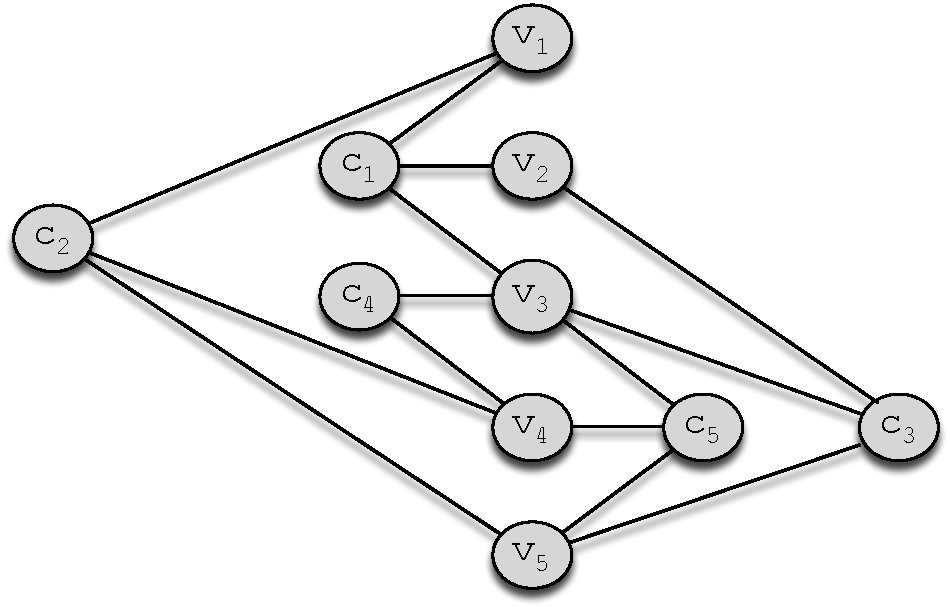
\includegraphics[scale=0.53]{figs/gvarphi.pdf}
% \caption{$G(\varphi)=(V(\varphi),E(\varphi))$ formed from $\varphi$ in Equation (\ref{eqn:varphi}) }
% \label{fig:gvarphi}
% \end{figure}

 
\begin{figure}[t]
  \begin{center}
    \fbox{\subfigure[Variable gadget $V_i$.The dashed edges are connections to clause gadgets.]{\label{fig:variable-gadget}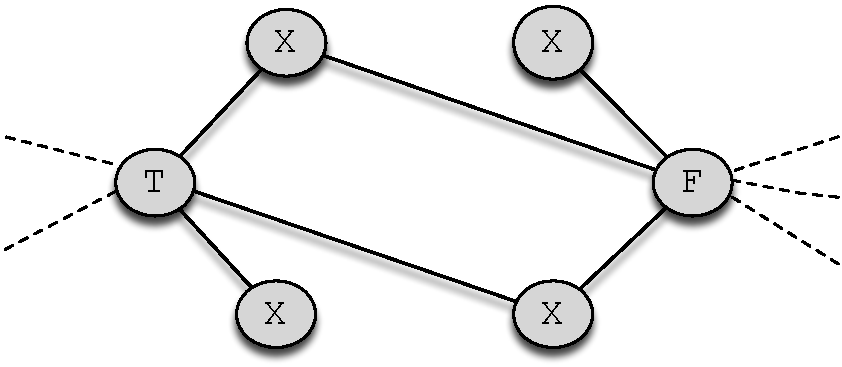
\includegraphics[scale=0.49]{figs/variable-gadget.pdf}}}
    \fbox{\subfigure[Clause gadget $C_j$. The dashed edges are connections to variable gadgets.]{\label{fig:clause-gadget}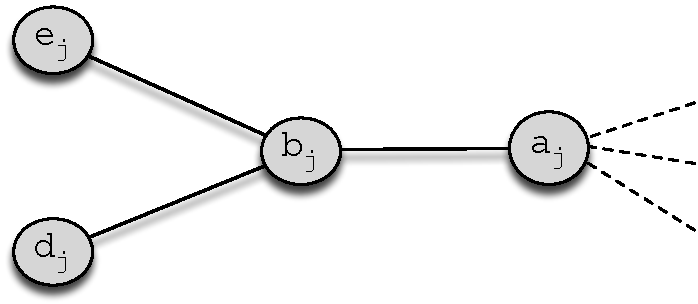
\includegraphics[scale=0.49]{figs/proof1b.pdf}}}
  \end{center}
	\caption{Gadgets used in Theorem \ref{thm:npc-maxinc} proof.}
  \label{fig:maxinc}
\end{figure}

%\begin{figure}[t]
%\centering
%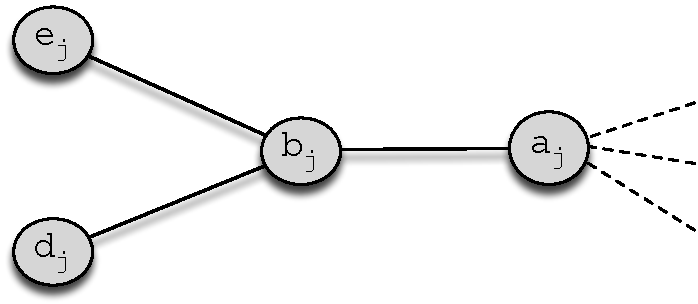
\includegraphics[scale=0.41]{figs/proof1b.pdf}
%\caption{Clause gadget, $C_j$, used in Theorem \ref{thm:npc-maxinc} proof.} 
%\label{fig:proof1}
%\end{figure}

\begin{figure}[t]
\centering
\includegraphics[scale=0.73]{figs/proof1b-example.pdf}
%\includegraphics[scale=0.51]{figs/example2.pdf}
\caption{Graph $G=(V,E)=H_1(\varphi)$ formed from $\varphi$ formula in Theorem \ref{thm:npc-maxinc} proof.} 
\label{fig:proof1-example}
\end{figure}

\begin{theorem}
\maxinc is NP-Complete. %even when restricted to the class of bipartite planar graphs.
\label{thm:npc-maxinc}
\end{theorem}

{\bf Proof idea:} First, we construct problem-specific gadgets for variables and clauses. We then demonstrate that any solution that observes $m$ nodes must place the PMUs only on nodes in the variable gadgets. Next we show that as a result of this, the problem of observing $m$ nodes in this graph reduces to the NP-complete problem presented in \cite{Brueni05}, which concludes our proof.

\begin{proof}
%\maxinc is easily in $\in \mathcal{NP}$. 
We start by arguing that \maxinc $\in \mathcal{NP}$. First, nondeterministically select $k$ nodes in which to place PMUs. Then we use the rules specified in Section \ref{subsec:observe} to determine
the number of observed nodes. 
%Haynes et al. \cite{Haynes02} show that given a PDS solution can be verified in polynomial time. Since \maxinc only checks $m < |V|$ vertices, 
%the same algorithm can be used to verify a \maxinc solution in polynomial time.

We reduce from \sats, where $\phi$ is an arbitrary \sat formula, to show \xval is NP-hard.
Note that $\phi$ is different from the example $\varphi$ formula used to introduce the \sat problem.
Specifically, given a graph $G(\phi)$ we construct a new graph $H_1(\phi) = (V_1(\phi), E_1(\phi))$ by replacing each variable 
(clause) node in $G(\phi)$ (Figure \ref{fig:gvarphi}) with the variable (clause) gadget shown in Figure \ref{fig:variable-gadget} (\ref{fig:clause-gadget}). The edges connecting clause gadgets 
with variable gadgets express which variables are in each clause: for each clause gadget $C_j$, node $a_j$ is attached to node $T$ in variable gadget $V_i$ if, in $\phi$, $v_i$ is in $c_j$,
and to node $F$ if $\overline{v_i}$ is in $c_j$. The resulting graph for the example given in Figure \ref{fig:gvarphi} is shown in Figure \ref{fig:proof1-example}; the corresponding formula 
for this graph, $\varphi$,
is satisfied by truth assignment $A_{\varphi}$: $\overline{v_1}, \overline{v_2}, v_3, \overline{v_4},$ and $\overline{v_5}$ are True. This corresponds to the dark shaded nodes in Figure
\ref{fig:proof1-example}. 
We also note that $H_1(\phi)$ is identical to the graph $H(\phi)$ constructed in \cite{Brueni05}, except that there $C_j$ consisted only of nodes $\{a_j,b_j\}$, and
thus $|H_1(\phi)| = |H(\phi)| + 2s$.  We return to this similarity later in the proof. For convenience, we let $G=H_1(\phi)$.

% Before beginning our proof that \maxinc is NP-hard, we briefly summarize the reduction from \sat used in \cite{Brueni05}. 
% Given a \sat formula, $\phi$, with variables $\{v_1,v_2, \dots , v_r\}$ and the set of
% clauses $\{c_1,c_2, \dots , c_s \}$, a graph $H(\phi) = (V(\phi),E(\phi))$ is formed as follows.  Each variable, $v_i$, is replaced with a gadget shown in Figure \ref{fig:variable-gadget}.  Each
% clause, $c_j$, is replaced with a 2-clique $C[j],C'[j]$.  The edges in $E(\phi)$ represent whether a clause contains a variable.  If the variable $v_i$ occurs in clause $c_j$, $C[j]$ is connected to 
% $v_i$'s $T$ node. Conversely, if $\overline{v_i}$ occurs in clause $c_j$, then $C[j]$ is connected to $v_i$'s $F$ node. 
% Figure \ref{fig:proof1-example} shows the graph $H(\varphi)$ formed from \sat formula $\varphi$, defined in Equation (\ref{eqn:varphi}), with one exception: 
% for each clause gadget, $C_j$, $C_j$'s two leaf nodes are removed.

% In our proof, we define the same \sat formula, $\phi$, as in \cite{Brueni05}: $\phi$ has variables $\{v_1,v_2, \dots , v_r\}$ and the set of clauses $\{c_1,c_2, \dots , c_s \}$.
% From $\phi$, we create a graph $G=(V,E)$ which is identical to $H(\phi)$ defined in \cite{Brueni05} with one exception. We replace each 2-clique $\{C[j],C'[j]\} \in H(\phi)$ with
% clause gadget $C_j$. Each $C_j$ has the following $\Gamma$ functions: $\Gamma(d_j) = \{b_j\}$, $\Gamma(e_j) = \{b_j\}$, $\Gamma(b_j) = \{a_j,d_j,e_j\}$, and $\Gamma(a_j) = \Gamma_o(C[j]) \cup \{b_j\}$
% where $\Gamma_o(C[j])$ is the $\Gamma$ function for $C[j] \in H(\phi)$. $C_j$ is shown in Figure \ref{fig:clause-gadget}.  

% For example, the graph for formula $\varphi$ defined in Equation (\ref{eqn:varphi}) is shown in Figure \ref{fig:proof1-example}.
% $\varphi$ is satisfied by truth assignment $A_{\varphi}$: $\overline{v_1}, \overline{v_2}, v_3, \overline{v_4},$ and $\overline{v_5}$ are true. 
% The dark shaded nodes have PMUs and correspond to $A_{\varphi}$.

With this construct in place, we move on to our proof. Here we consider the case of  $k=r$ and $m = 6r + 2s$, and show that $\phi$ is satisfiable if and only if $r=|\Phi_G|$ PMUs 
can be placed on $G$ such that $m \leq |\Phi^R_{G}| < |V|$. We will later discuss how to extend this proof for any larger value of $m$.  %cover $m$ nodes in $G'$.

$(\Rightarrow)$ Assume $\phi$ is satisfiable by truth assignment $A_{\phi}$. Then, consider the placement $\Phi_G$ s.t. for each variable gadget $V_i$, $T_i\in \Phi_G \Leftrightarrow v_i=True$ 
in $A_\phi$, and  $F_i\in \Phi_G \Leftrightarrow v_i=False$. It has been shown in \cite{Brueni05} that for $H(\phi)$ this placement observes all $H(\phi)$, and it can be easily verified that
all nodes in $H_1(\phi)$ are observed as well except for $d_j, e_j$ for each $C_j$. This amounts to $2s$ nodes, so exactly $m$ nodes are observed by $\Phi_G$, as required.  

$(\Leftarrow)$ 
We begin by proving that any solution that observes $m$ nodes must place the PMUs only on nodes in the variable gadgets. Assume that there are $1<t\leq r$ variable gadgets without a PMU. 
Then, at most $t$ PMUs are on nodes in clause gadgets, so {\it at least} $\max(s-t,0)$ clause gadgets are without PMUs. We want to show here that for $m=6r+2s$, $t=0$.

To prove this, we rely on the following two simple observations:
\begin{itemize}
	\item In any variable gadget $V_i$, nodes $X$ (Figure \ref{fig:variable-gadget}) cannot be observed unless  there is a PMU somewhere in $V_i$. Note that there are $4$ such nodes per $V_i$.
	\item In any clause gadget $C_j$, nodes $e_j$ and $d_j$ cannot be observed unless there is a PMU somewhere in $C_j$. Note that there are $2$ such nodes per $C_j$. 
\end{itemize}
Thus, given some $t$, the number of unobserved nodes is {\it at least} $4t + \max(2(s-t), 0)$. However, since $|V|-m \leq 2s$, there are {\em at most}  $2s$ unobserved nodes. So we get 
$2s \geq 4t + \max(2(s-t), 0)$. We consider two cases:
\begin{itemize}
	\item $s\geq t$: then we get $2s \geq 2s+2t \Rightarrow t=0.$
	\item $s < t$:	then we get $2s \geq 4t \Rightarrow s\geq 2t$, and since we assume here $0\leq s < t$ this leads to a contradiction and so this case cannot occur.
\end{itemize}

Thus, we have concluded that the $r$ PMUs must be on nodes in variable gadgets, all of which, it is important to note, were also part of the original $H(\phi)$ graph. 
We return to this point shortly. 

We now observe that for each clause gadget $C_j$, such a placement of PMUs cannot observe nodes of type  $e_j, d_j$, which amounts to a total of $2s$ unobserved nodes - the allowable bound.
This means that all other nodes in $G$ must be observed. Specifically, this is exactly all the nodes in the original $H(\phi)$ graph, and PMUs can only be placed on variable gadgets, 
all of which are included in $H(\phi)$ as well. Thus, the problem reduces to the problem in \cite{Brueni05}. 
We use the proof in \cite{Brueni05} to determine that all clauses in $\phi$ are satisfied by the truth assignment derived from $\Phi_G$. 
%which has already been proven that all clauses in $\phi$ are satisfied by the truth assignment derived from $\Phi_G$. 
\end{proof}
%Finally, we show that $G$ is bipartite and planar. From \cite{Brueni05} we know that $H(\phi)$ is bipartite and planar.  Recall, the only difference between $G$ and $H(\phi)$ is that $G$'s clause
%gadgets have two extra nodes: $d_j$ and $e_j$.  We must show that the addition of all $d_j$ and $e_j$ to $H(\phi)$ maintains the condition that the resulting graph, $G$, is bipartite and planar. 
%We add $d_j$ and $e_j$ to the same partition as $a_j$, $V_1$. 
%Because $d_j$ and $e_j$ are only connected to $b_j$ and $b_j \notin V_1$, 
%this maintains the condition that $G$ is bipartite. 

%By definition every \sat formula, $\phi$, has a planar embedding $G(\phi)$.  From \cite{Brueni05} we know that $H(\phi)$ maintains the planar
%embedding. By inspection, adding $d_j$ and $e_j$ to $H(\phi)$ preserves the condition that $G$ is planar.
%\end{proof}


\subsection{\xval Problem Statement}
\label{subsec:xval}

%First we dedine \xval as an optimization problem and then state then state the \xval as a decision problem. 

\xval Optimization Problem:
\begin{itemize}
	\item \underline{Input}: Graph $G=(V,E)$.
	%\item \underline{Input}: Graph $G=(V,E)$ and $k$ PMUs.

	\item \underline{Output}: A placement of PMUs, $\Phi_G$, such that $\Phi^R_G = V$,
	 each $v \in \Phi_G$ is cross-validated according to the rules specified in Section \ref{subsec:xval}, and  $\Phi_G$ is minimal.
\end{itemize}

\xval Decision Problem:
\begin{itemize}
	\item \underline{Instance}: Graph $G=(V,E)$, $k$ PMUs such that $k \geq 1$.

	\item \underline{Question}: Is there a $\Phi_G$ such that $|\Phi_G| \leq k$, $\Phi^R_G = V$, and each $v \in \Phi_G$ is cross-validated?  
	%\item \underline{Question}: Is there a $\Phi \subseteq V$ such that $|\Phi| \leq k$, $\Phi^R = V$, and each $\phi \in \Phi$ is cross-validated?  
\end{itemize}

\begin{figure}[t]
\centering
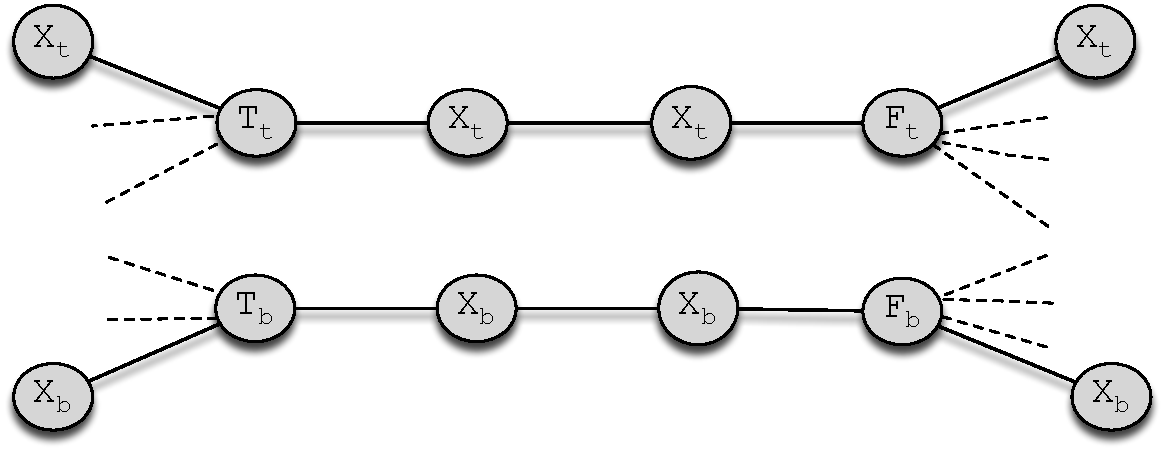
\includegraphics[scale=0.55]{figs/xvalgadget2.pdf}
%\includegraphics[scale=0.51]{figs/example2.pdf}
\caption{Variable gadget used in Theorem \ref{thm:npc-xval} proof. The dashed edges are connections to clause gadgets.} 
\label{fig:xval-gadget}
\end{figure}

\begin{theorem}
\xval is NP-Complete. % even when restricted to the class of bipartite and chordal graphs.
\label{thm:npc-xval}
\end{theorem}

% {\bf Proof idea:} We show \xval is NP-hard by reducing from \sats.  Similar to our redcution
% for \maxincs, we create a clause gadget for each clause in \sat forumula, $\phi$, and a variable gadget 
% for each variable in $\phi$.  The clause gadget is a pair of nodes connected by an edge.  The variable 
% gadget is shown in Figure \ref{fig:xval-gadget}.  A variable gadget, $V_i$, is connected to the clause gadgets, $C_j$, only if 
% variable $v_i$ appears in clause $c_i$ in $\phi$.
% 
% %If a variable, $v_i$, appears in clause, $c_j$, 
% %$c_j$'s clause gadget has the edges $(C[j], T_t), (C[j],T_b)$. Similarily, if clause $c_j$ 
% %contains variable $\overline{v_i}$ in $\phi$, the $c_j$'s clause gadget has the edges $(C[j], F_t), (C[j],
% %F_b)$.
% 
% We place PMUs on variable gadget nodes $T$ and $F$ according to the literal value of each variable in the satisfying truth assignment for $\phi$. 
% %PMUs at $T$ nodes are cross-validated using XV2 via the common clause node. 
% This leads to a fully observed graph in which all PMUs are cross-validated.  In the other direction, we show that $G$ can only be fully observed
% if $2$ PMUs are placed on each variable gadget. Specifcally, PMUs must be placed on both $T$ nodes or both $F$ nodes, in each variable gadget.  We use the PMU placement
% to derive a satisfying truth assignment for \sat formula $\phi$.
%All clause nodes are observed because each clause is adjacent to at least one PMU node.  The variable clauses are 
%Given a satisfying truth assingment to $\phi$, we place PMUs $T$ nodes and $F$ nodes only. 
%If a variable $v_i \in \phi$ is True, we place a PMU on each of the $T$ nodes of $v_i$ corresponding variable gadget.  Likewise,
%if $v_i$ is false, a PMU is placed on the $F$ nodes of $v_i$'s variable gadget.  

% variable gadgets and clause gadgets 
% => place PMUs on T/F nodes of each variable gadget
% <= in order for G to be fully observed each variable gadget must have 2 PMUs,  in order to satisfy cross-validation
%   must be on T/F nodes.  PMU on T node implies variable is true and vice versa.  in this way we derive a satisfying assignment for $\phi$
% 


\begin{proof}
First, we argue that \xval $\in \mathcal{NP}$.  Given a \xval solution, we use
the polynomial time algorithm described in our proof for Theorem
\ref{thm:npc-maxinc} to determine if all nodes are observed.  Then, for each
PMU node we run a breadth-first search, stopping at depth $2$, to check that
the cross-validation rules are satisfied.

To show \xval is NP-hard, we reduce from \sats.  Our reduction is similar to
the one used in Theorem \ref{thm:npc-maxinc}.  
% Given a \sat formula, $\phi$,
% with variables $\{v_1,v_2, \dots , v_r\}$ and the set of clauses $\{c_1,c_2,
% \dots , c_s \}$, we form a new graph, $G=(V,E)$, as follows. Each clause $c_j$
% corresponds to a pair of nodes connected by an edge, denoted $C[j],C'[j]$. This
% is the same construct as described in the original proof \cite{Brueni05}. 
For this problem, we use different variable and clause gadgets. The clause gadgets consist of the edge $(a_j, b_j)$ from Figure \ref{fig:clause-gadget},
which are the same as used in \cite{Brueni05}. The new variable gadget is shown in Figure
\ref{fig:xval-gadget}. As can be seen in this figure, the variable gadgets are comprised of two disconnected
subgraphs: we refer to the upper subgraph as $V_{it}$ and the
lower subgraph as $V_{ib}$. Clause gadgets are connected to a variable gadgets in the following manner: 
for each clause $c_j$ that contains variable $v_i$ in $\phi$, the corresponding clause gadget has the edges $(a_j, T_t), (a_j,
T_b)$, and for each clause $c_j$ that contains variable $\overline{v_i}$ in
$\phi$, the corresponding clause gadget has the edges $(a_j, F_t), (a_j,
F_b)$. We denote the resulting graph as $H_2(\phi)$, and for what follows assume $G=H_2(\phi)$.

%Let $k = 2r$. 
We now show that $\phi$ is satisfiable if and only if
$k=2r$ PMUs can be placed on $G$ such that $G$ is fully observed under the
condition that all PMUs are cross-validated, and that $2r$ PMUs are the minimal 
bound for observing the graph with cross-validation.

$(\Rightarrow)$ Assume $\phi$ is satisfiable by truth assignment $A_{\phi}$.
For each $1\leq i\leq r$, if $v_i=True$ in $A_{\phi}$ we place a PMU at $T_b$
and at $T_t$ of the variable gadget $V_i$. Otherwise, we place a PMU at $F_b$
and at $F_t$ of this gadget. In either case, the PMU nodes in $V_i$ must be
adjacent to a clause node, making $T_t$ ($F_t$) two hops away from
$T_b$ ($F_b$). Therefore, all PMUs are cross-validated by XV2. 

Now we argue that $\Phi_G$ observes all $v \in V$:  
\begin{itemize}
  \item Consider a clause node $a_j$. Since $\phi$ is satisfied, for some
  index $i$ we have  $v_i \in c_j \wedge v_i\in A_{\phi}$ or $\overline{v_i} \in
  c_j \wedge \overline{v_i}\in A_{\phi}$. For the first case, the PMUs in $V_i$ are placed
  on $\{T_b, T_t\}$ and as a result $a_j$ is observed by applying O1 at $T_b$ or at  $T_t$. A similar argument applies for the second case. So, all $a_j$
  nodes are observed.

  \item Next, consider the nodes on the variable gadgets.  When $v_i \in A_{\phi}$,
  $T_t$'s neighbors, in $V_{it}$, are observed via O1.
  (the second case, $\overline{v_i} \in A_{\phi}$, follows by symmetry). 
  The remaining $V_{it}$ nodes are observed via O2 - note that if $F_t$ is connected to a clause gadget we know from the previous step this clause is observed. By symmetry of $V_{ib}$ and
  $V_{it}$, the same argument can be made for $V_{ib}$ to show all $V_{ib}$ nodes
  are observed.

 \item Finally, all the neighbors of $a_j$ in variable gadgets are observed, and $a_j$ is observed, so we can now apply O2 at each node $a_j$ to observe the remaining $b_j$ nodes.
\end{itemize}
This completes this direction of the theorem.

$(\Leftarrow)$ Suppose $\Phi_G$ observes all nodes in $G$
under the condition that each PMU is cross-validated, and that $|\Phi_G|=2r$. We want to show that
$\phi$ is satisfiable by the truth assignment derived from $\Phi_G$. We prove this by showing
that (a) each variable gadget must have exactly $2$ PMUs and (b) there must be
a PMU at each subgraph of the variable gadget. Once (b) is shown, (c)
cross-validation restrictions force the PMUs to be either on both
$T$-nodes or both $F$-nodes. We conclude by showing that (d) the PMU nodes correspond
to true/false assignments to variables which satisfy $\phi$.

We begin by showing that each variable gadget must have $2$ PMUs. Let
$V_i$ be a variable gadget with less than two PMUs. By placing PMUs on
clause gadgets attached to $V_i$, at most we can observe $T_t, T_b, F_t$ and
$F_b$ directly from the clause gadgets. Next, at least one of the $V_i$
subgraphs has no PMU: without loss of generality, let this be $V_{it}$. 
We cannot apply O1 at $T_t$ or $F_t$,
since they have no PMU. We cannot apply O2 at these nodes since they each have
two unobserved $X_t$ nodes. Thus, all $X_t$ nodes are unobserved in $V_{it}$,
contrary to our assumption that the entire graph is observed. Thus we have
shown that there must be at least $2$ PMUs at each variable gadget. Also 
it is clear from this proof that, in fact, there must be at least one PMU in each subgraph of each
variable gadget. Finally, since there are $2r$ PMUs and $r$ variables, we conclude that 
each variable gadget has exactly two PMUs -- one PMU for each variable gadget subgraph --
and there are no PMUs on clause nodes.
%accounts for all the PMUs - no PMUs on clause nodes.

Due to the cross-validation constraint, it is clear that a PMU on $V_{it}$ can only
be cross-validated by a PMU on $V_{ib}$ (since all other variable-gadgets are
more than $2$ hops away), and specifically this would require both to be either
on $\{T_t, T_b\}$ or $\{F_t, F_b\}$. 

Without loss of generality, assume for an arbitrary variable gadget, $V_i$, 
we placed the PMUs at $\{T_t, T_b\}$. By applying O1 and O2, this
placement can observe all nodes in the variable gadget if $\{F_t, F_b\}$ in this gadget
are not adjacent to a clause node. If they are adjacent to some $a_h$ node, each of $\{F_t, F_b\}$ can observe its adjacent leaf-$X$-node only via O2, and only if
$a_h$ is already observed. Since we are given a PMU placement that observes the entire
graph, this implies that $a_h$ is indeed observed and thus adjacent to some variable node with a PMU,
such that O1 could be applied to view $a_h$. Assume without loss of generality,
$a_h$ is adjacent to PMU nodes $T_b,T_t$ from variable gadget $V_l$, then the clause $c_h \in \phi$ is
satisfied if $v_l$ is true. A similar argument can be made if $V_l$ is adjacent to
PMU nodes $F_t, F_b$. We conclude that all clauses in $\phi$ are satisfied by
the truth assignment derived from $\Phi_G$.
\end{proof}


\subsection{\xvalpart Problem Statement}
\label{subsec:xvalpart}

\xvalpart Optimization Problem:
\begin{itemize}

	\item \underline{Input}: Graph $G=(V,E)$ and $k$ PMUs  such that $1 \leq k < k^*$.

	\item \underline{Output}: A placement of $k$ PMUs, $\Phi_G$, such that $|\Phi^R_G|$ is maximum under the condition that 
	each $v \in \Phi_G$ is cross-validated according to the rules specified in Section \ref{subsec:xval}.
\end{itemize}


\xvalpart Decision Problem:
%Given $k < k^*$ PMUs, is there a $\Phi \subseteq V$ such that $|\Phi| \leq k$ and $|\Phi^R| \geq m$?
\begin{itemize}
	\item \underline{Instance}: Graph $G=(V,E)$, $k$ PMUs such that $1 \leq k < k^*$, and some $m<|V|$.

	\item \underline{Question}: Is there a $\Phi_G$ such that $|\Phi_G| \leq k$, $m \leq|\Phi^R_G| < |V|$ under the condition that each $v \in \Phi_G$ is cross-validated?
	%\item \underline{Question}: Is there a $\Phi \subseteq V$ such that $|\Phi| \leq k$, $m \leq|\Phi^R| < |V|$, and each $\varphi \in \Phi$ is cross-validated?
\end{itemize}

\begin{theorem}
\xvalpart is NP-Complete. % even when restricted to the class of bipartite and chordal graphs.
\label{thm:npc-xvalpart}
\end{theorem}

%{\bf Proof Idea:} We show \xvalpart is NP-hard by reducing from \sats. Our proof is a combination of the techniques introduced in the NP-hardness proofs for \maxinc and \xvals,
%and is presented here at a high-level only with the details left to the reader to verify.\\ 
%From a \sat formula, we create a graph $G$ with the clause gadgets from \maxinc (Figure \ref{fig:clause-gadget}) and the variable gadgets from \xval (Figure \ref{fig:xval-gadget}).
%The edges in $G$ connecting clause and variable gadgets are the same as in $H_2(\varphi)$, and consider a proof with $m = |V|-2s$ as with \maxinc. 

{\bf Proof Idea:} We show \xvalpart is NP-hard by reducing from \sats. Our proof is a combination of the NP-hardness proofs for \maxinc and \xvals.  Due to space constraints,
From a \sat formula, $\phi$, we create a graph $G=(V,E)$ with the clause gadgets from \maxinc (Figure \ref{fig:clause-gadget}) and the variable gadgets from \xval (Figure \ref{fig:xval-gadget}).
The edges in $G$ are identical the ones the graph created in our reduction for \xvals. 

We show that any solution that observes $m=|V|-2s$ nodes must place the PMUs exclusively on nodes in the variable gadgets. As a result, we show
$2$ nodes in each clause gadget -- $e_j$ and $d_j$ for clause $C_j$ -- are not observed, yielding a total $2s$ unobserved nodes. This implies all other nodes must be 
observed, and thus reduces our problem to the scenario considered in Theorem \ref{thm:npc-xval}, which is already proven.


\begin{proof}
\xvalpart is easily in $\mathcal{NP}$. We verify a \xvalpart solution using the same polynomial time algorithm described in our proof 
for Theorem \ref{thm:npc-xval}. % used to verify an \xval solution.

We reduce from \sat to show \xvalpart is NP-hard. Our reduction is a combination
of the reductions used for \maxinc and \xvals. Given a \sat formula, $\phi$,
with variables $\{v_1,v_2, \dots , v_r\}$ and the set of clauses $\{c_1,c_2,
\dots , c_s \}$, we form a new graph, $H_3(\phi) = (V(\phi),E(\phi))$  as follows. Each clause $c_j$
corresponds to the clause gadget from \maxinc (Figure \ref{fig:clause-gadget}) 
and the variable gadgets from \xval (Figure \ref{fig:xval-gadget}). 
As in Theorem \ref{thm:npc-xval}, we refer to the upper subgraph of variable gadget, $V_i$, 
as $V_{it}$ and the lower subgraph as $V_{ib}$.  Also, we let $H_3(\phi) = G=(V,E)$.

Let $k = 2r$ and $m = 12r + 2s = |V| - 2s$. As in our NP-hardness proof for \maxincs, $m$ includes all nodes in $G$
except $d_j,e_j$ of each clause gadget. We need to show that $\phi$ is satisfiable if and only if
$2r$ cross-validated PMUs can be placed on $G$ such that $m \leq |\Phi^R_{G}| < |V|$.

$(\Rightarrow)$ Assume $\phi$ is satisfiable by truth assignment $A_{\phi}$.
For each $1\leq i\leq r$, if $v_i=True$ in $A_{\phi}$ we place a PMU at $T_b$
and at $T_t$ of the variable gadget $V_i$. Otherwise, we place a PMU at $F_b$
and at $F_t$ of this gadget. In either case, the PMU nodes in $V_i$ must be
adjacent to a clause node, making $T_t$ ($F_t$) two hops away from
$T_b$ ($F_b$). Therefore, all PMUs are cross-validated by XV2. 

This placement of $2r$ PMUs, $\Phi_G$, is exactly the same one derived from $\phi$'s satisfying instance in Theorem \ref{thm:npc-xval}.
Since $\Phi_G$ only has PMUs on variable gadgets, all $a_j$ and $b_j$ nodes are observed by the same argument used in Theorem \ref{thm:npc-xval}.
Thus, at least $12r + 2s$ nodes are observed in $G$.
Because no PMU in $\Phi_G$ is placed on a clause gadget, $C_j$, we know that all $e_j$ and $d_j$ are not observed. 
We conclude that exactly $m$ nodes are observed using $\Phi_G$.

$(\Leftarrow)$ 
We begin by proving that any solution that observes $m$ nodes must place the PMUs only on nodes in the variable gadgets. Assume that there are $1<t\leq r$ variable gadgets without a PMU. 
Then, at most $t$ PMUs are on nodes in clause gadgets, so {\it at least} $\max(s-t,0)$ clause gadgets are without PMUs. We want to show here that for $m=12r+2s$, $t=0$.

To prove this, we rely on the following observations:
\begin{itemize}
	\item As shown in Theorem \ref{thm:npc-xval}, a variable gadget's subgraph with no PMU has at least $4$ unobserved nodes.
	\item In any clause gadget $C_j$, nodes $e_j$ and $d_j$ cannot be observed if there is no PMU somewhere in $C_j$. Note that there are $2$ such nodes. 
\end{itemize}
Thus, given some $t$, the number of unobserved nodes is {\it at least} $4t + \max(2(s-t), 0)$. However, since $|V|-m \leq 2s$, there are {\em at most}  $2s$ unobserved nodes. So we get 
$2s \geq 4t + \max(2(s-t), 0)$. We consider two cases:
\begin{itemize}
	\item $s\geq t$: then we get $2s \geq 2s+2t \Rightarrow t=0.$
	\item $s < t$:	then we get $2s \geq 4t \Rightarrow s\geq 2t$, and since we assume here $0\leq s < t$ this leads to a contradiction and so this case cannot occur.
\end{itemize}

Thus, we have concluded that the $2r$ PMUs must be on variable gadget. %, which, it is important to note, were also part of the original $H(\phi)$ graph. We shall return to this point shortly. 
We now observe that for each clause gadget $C_j$, such a placement of PMUs cannot observe nodes of type  $e_j, d_j$, which amounts to a total of $2s$ unobserved nodes - the allowable bound.
This means that all other nodes in $G$ must be observed. Specifically this is exactly all the nodes in $H_2(\phi)$ from the Theorem \ref{thm:npc-xval} proof, and PMUs can only be placed on 
variable gadgets, all of which are included $H_2(\phi)$ from the Theorem \ref{thm:npc-xval} proof. Thus, the problem reduces to the problem in Theorem \ref{thm:npc-xval} and so we 
the Theorem \ref{thm:npc-xval} proof to determine that all clauses in $\phi$ are satisfied by the truth assignment derived from $\Phi_G$. 
\end{proof}



\subsection{Extending Gadgets to Cover a Range of $m$ and $|V|$ values}
\label{subsec:extend}

In the \xvalpart and \maxinc proofs we demonstrated NP-completeness for $m=|V|-2s$. 
We show that slight adjustments to the variable and clause gadgets can yield a much wider range of $m$ and $|V|$ values. 
We present the outline for new gadget constructions and leave the detailed analysis to the reader.

To increase the size of $m$ (e.g., the number of observed nodes), we simply add more $X$ nodes between the $T$ and $F$ nodes in the variable gadgets used in our proofs for \xvalpart and \maxincs. 
The new variable gadgets for \maxinc and \xvalpart are shown in Figure \ref{fig:variable-extend1} and Figure \ref{fig:variable-extend2}, respectively.
The same PMU placement described in the NP-Completeness proofs for each problem observes these newly introduced nodes.

%In order to increase the size of $|V|$ while keeping $m$ the same, we modify the clause gadget by repeatedly adding a pair $b_{j,h}, d_{j,h}$ of leaves rooted 
%at $d_{j,h-1}$, where $d_j = d_{j,0}, b_j = b_{j,0}$, for $h\rightarrow \infty$.  
In order to increase the size of $|V|$ while keeping $m$ the same, we replace each clause gadget, $C_j$ for $1 \leq j \leq s$, with a new clause gadget, $C_j'$,
shown in Figure \ref{fig:clause-extend}.  %We refer to the new clause gadget as $C_j'$.
For \maxincs, the optimal placement of PMUs on $C_j'$ is to place PMUs on every fourth $b_{j,h}$ node, as shown in Figure \ref{fig:clause-extend-observe}. 
%As a result, half of the $d_{j,h}$ nodes are observed via O2 as shown in Figure \ref{fig:clause-extend-observe}. 
As a result, the optimal placement of $l$ PMUs on $C_j'$ can at most observe $6l$ nodes.  By adding $6l$ $T$ nodes to each variable gadget, more nodes 
are always observed by placing a PMU on the variable gadget rather than at a clause gadget. We can use this to argue that PMUs are only placed on variable gadgets and then leverage the 
argument from Theorem \ref{thm:npc-maxinc} to show \maxinc is NP-Complete for any $\frac{m}{|V|}$. A similar argument can be made for \xvalparts.

\begin{figure}[t]
  \begin{center}
    \subfigure[Extended variable gadget used for \maxincs.]{\label{fig:variable-extend1}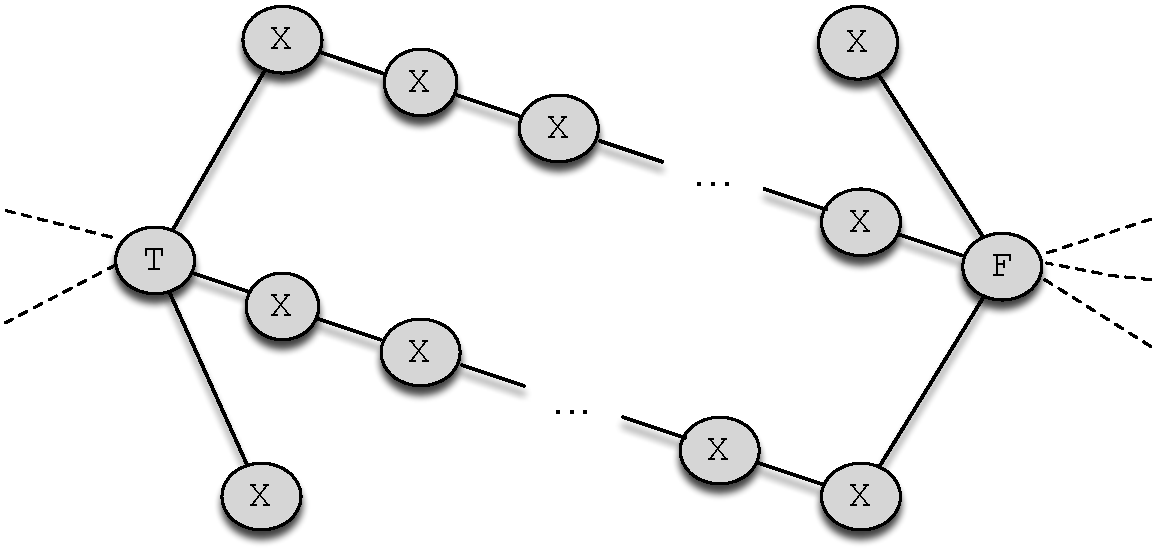
\includegraphics[scale=0.55]{figs/variable-gadget-extend.pdf}}
    \subfigure[Extended variable gadget used for \xvalparts.]{\label{fig:variable-extend2}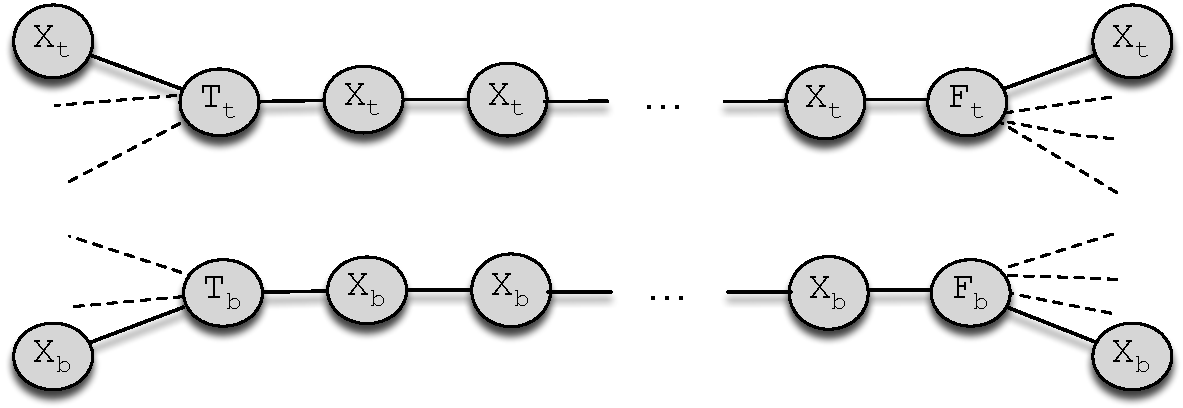
\includegraphics[scale=0.55]{figs/xvalgadget2-extend.pdf}}
  \end{center}
	\caption{Figures for variable gadget extensions described in Section \ref{subsec:extend}. The dashed edges indicate connections to clause gadget nodes. }
  \label{fig:clause-extended}
\end{figure}


\begin{figure}[t]
  \begin{center}
    \subfigure[Extended clause gadget $C_j$.]{\label{fig:clause-extend}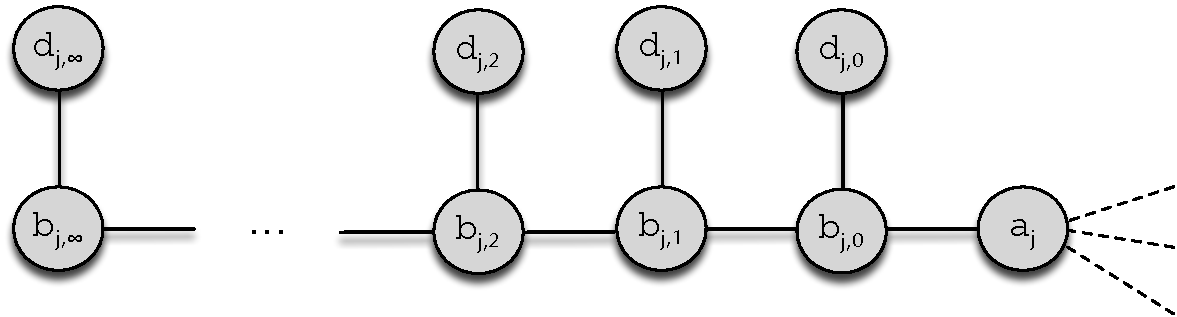
\includegraphics[scale=0.55]{figs/clausegadget-extension.pdf}}
    \subfigure[Observed nodes in extended clause gadget $C_j$ shown in (a).  PMU nodes are dark gray, nodes observe by O2 have a dashed border, and all other
	nodes are observed by O1.]
	{\label{fig:clause-extend-observe}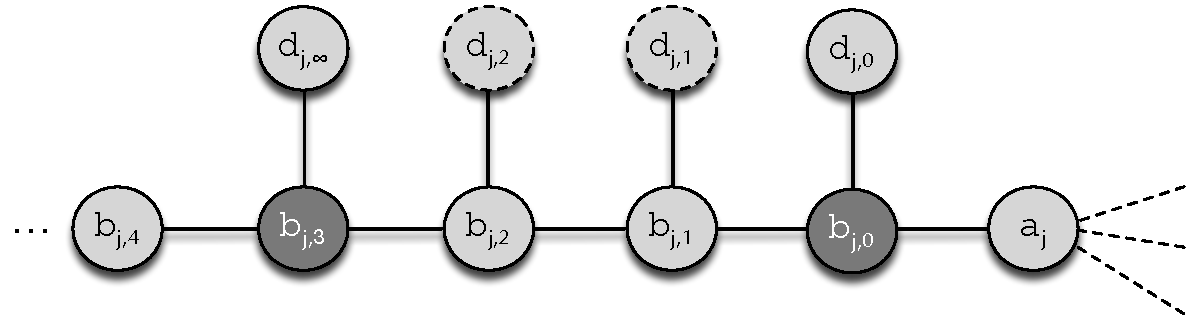
\includegraphics[scale=0.55]{figs/clausegadget-extension-observe.pdf}}
  \end{center}
	\caption{Figures for clause gadget extensions described in Section \ref{subsec:extend}. The dashed edges indicate connections to variable gadget nodes. }
  \label{fig:clause-extended}
\end{figure}

